\begin{frame}
    \frametitle{Solution concepts in games}
    \centering
    \[
        A \in \mathbb{R} ^ {m \times n}, \qquad B \in \mathbb{R} ^ {m \times n}   
    \]

    \pause
    \[
        \frac{dx}{dt}_i = x_i((f_x)_i - \phi_x), \quad \text{ for all }i
    \]
    \[
        \frac{dy}{dt}_i = y_i((f_y)_i - \phi_y), \quad \text{ for all }i
    \]
    
    \pause
    \tiny
    \vspace{1cm}
    \begin{itemize}
        \item Fudenberg, Drew, et al. The theory of learning in games. Vol. 2. MIT press, 1998.
        \item Elvio, Accinelli and Carrera, Edgar. 2011. Evolutionarily Stable Strategies and Replicator Dynamics in Asymmetric Two-Population Games. 10.1007/978-3-642-11456-4\_3.
    \end{itemize}

\end{frame}

\begin{frame}
    \frametitle{Inefficiency measure}

    \begin{equation*}
        PoA = \frac{\max_{s \in E} Cost(s)}{\min_{s \in S} Cost(S)}
    \end{equation*}
    \pause
    \footnotesize
    \vspace{1cm}
    \begin{equation*}
        PoA_A(s_r) = \frac{Cost(s_r)}{\min_{s \in S} Cost(S)}, \hspace{1cm} 
        PoA_B(s_c) = \frac{Cost(s_c)}{\min_{s \in S} Cost(S)}
    \end{equation*}

\end{frame}


\begin{frame}
    \frametitle{Learning algorithms - Asymmetric replicator dynamics}

    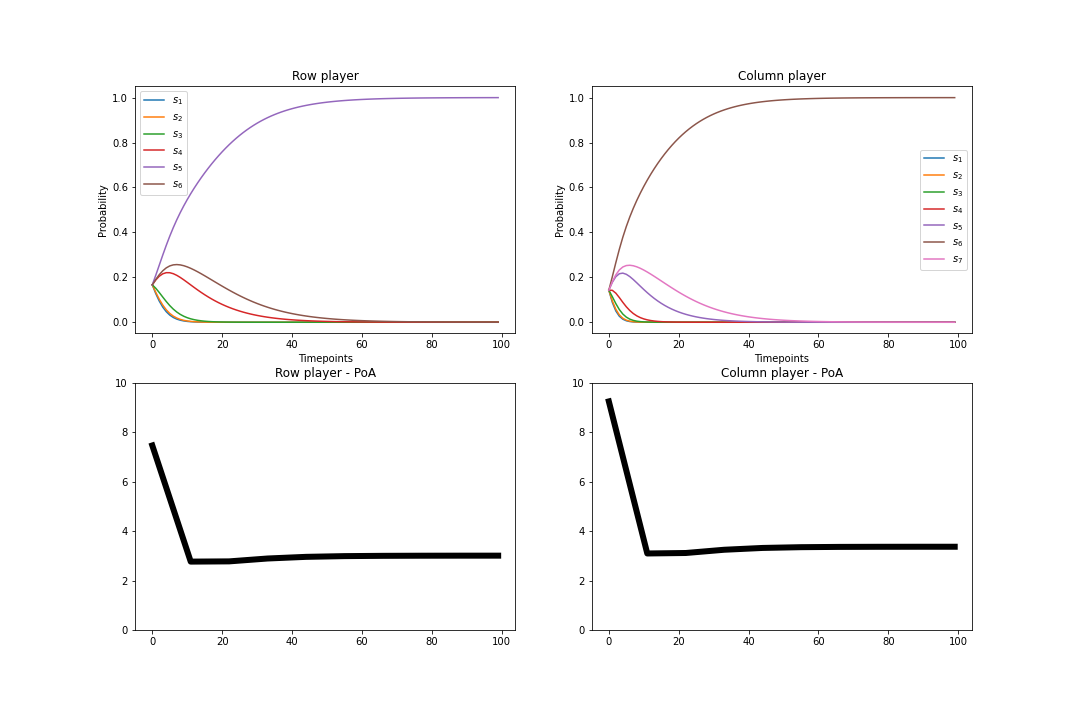
\includegraphics[scale=0.28]{Bin/ARD_game.png}
    
\end{frame}

\begin{frame}
    \centering
    \Huge{
    ``Inefficiencies can be learned and emerged naturally in an interactive system''
    }
\end{frame}


\begin{frame}
    \frametitle{Learning algorithms - Asymmetric replicator dynamics}

    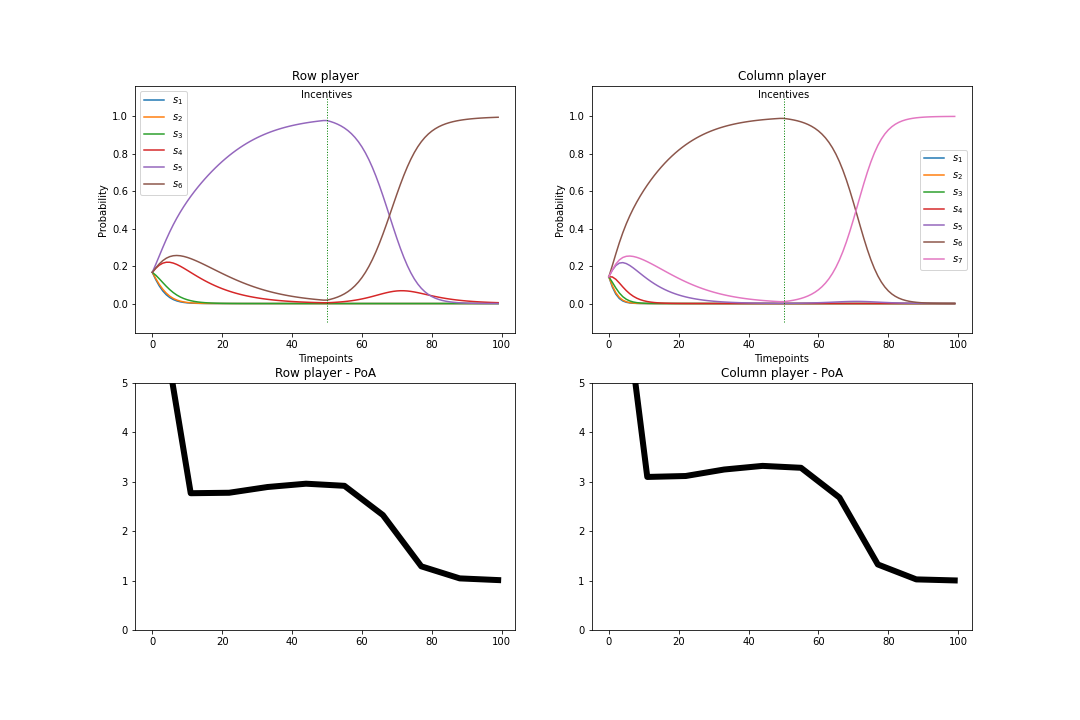
\includegraphics[scale=0.28]{Bin/ARD_penalty_game.png}
    
\end{frame}


\begin{frame}
    \centering
    \Huge{
    ``Targeted incentivisation of behaviours can help escape learned inefficiencies''
    }
\end{frame}
